\chapter{Result Discussion}

In this chapter, the obtained results are thoroughly analysed and discussed. The performed experiments can be subdivided into 6 categories: Curtail Lower Limit (section \ref{sec:curtailment-lower-limit}), Limit Infeasible Curtailment Actions \ref{sec:limit-infeasible}, Reward Tests\ref{sec:rewards}, \acp{GNN} Hyperparameter Tuning, \ac{GNN} Implementation Comparison \ref{sec:gnn-comparison} and Scability Tests \ref{sec:gnn-comparison}.

\begin{comment}
	* Best SAC and GNN parameters
	* Explain that SAC was used for most experiments as a baseline
\end{comment}

\section{Observation Space}

\
204.76815605163574,500,65.262,40.00237062805891,559046.9067760558,2302.7692077946244

\section{Issues with Curtailment Actions} \label{sec:limit-infeasible}

The initial exploratory experiments and posterior training performance analysis showed significant instability and lack of convergence of \ac{DRL} models. During the experimentation phase, the developed implementations, SAC and GCN-SAC, showed a significantly reduced survival rate. This posed a substantial problem since models failed to survive enough steps to appropriately learn economic policies, leading to relatively short results in their test phase. \par
Upon further research, the root of this problem was found to be related to the inclusion of curtailment actions, which made the action space more complex and, in turn, severely affected the models' performance. More specifically, during the exploratory phase, the abrupt changes in curtailment caused infeasible states of the system and, consequently, an early episode truncation.
Two methods were experimented to mitigate this problem, which are described in the following subsections.

\subsection{Limit Curtailment Infeasible States}

The first method that was analysing the effect of using the grid2op  \texttt{LIMIT\_INFEASIBLE\_CURTAILMENT\_STORAGE\_ACTION} parameter, which according to its own long name and documentation limits infeasible system states derivative from curtailment (and storage) actions. \par
For this purpose, three models were trained with the SAC and GCN-SAC models: 
\begin{itemize}
	\item Without curtailment
	\item With curtailment and without the parameter
	\item With curtailment and the parameter
\end{itemize}

\begin{comment}
	TODO -> LIMIT Experiements Graphs and tables
\end{comment}

The training results confirmed the initial suspicions, confirming that performance is significantly and negatively affected when including curtailment actions. However, when setting the \texttt{LIMIT\_INFEASIBLE\_CURTAILMENT\_STORAGE\_ACTION} the model was able to achieve notoriously higher results than any of the others on both training and test results. In table \ref{}, the results from the test phase can be observed.

\begin{figure}[H]
	\centering
	\subfloat{}{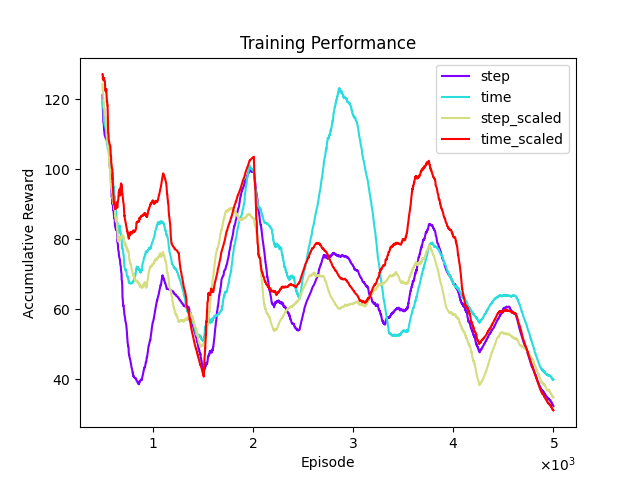
\includegraphics[width=.45\textwidth]{graphs/obs/training_performance.png}}
	\hskip1ex
	\subfloat{}{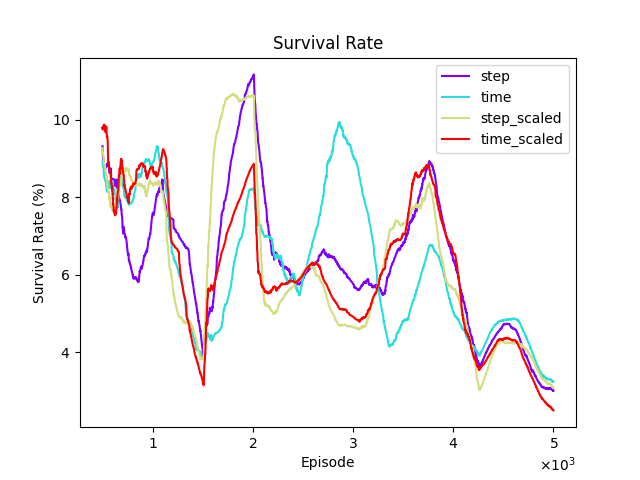
\includegraphics[width=.45\textwidth]{graphs/obs/survival_rate.png}} 
	\vfill
	\subfloat{}{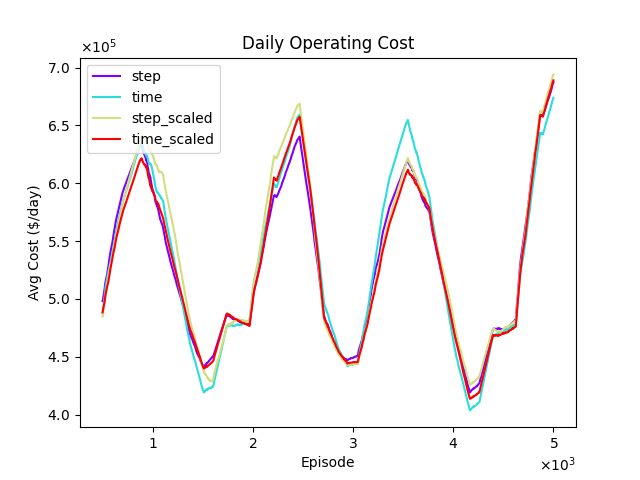
\includegraphics[width=.45\textwidth]{graphs/obs/daily_cost.png}} \hskip1ex
	\subfloat{}{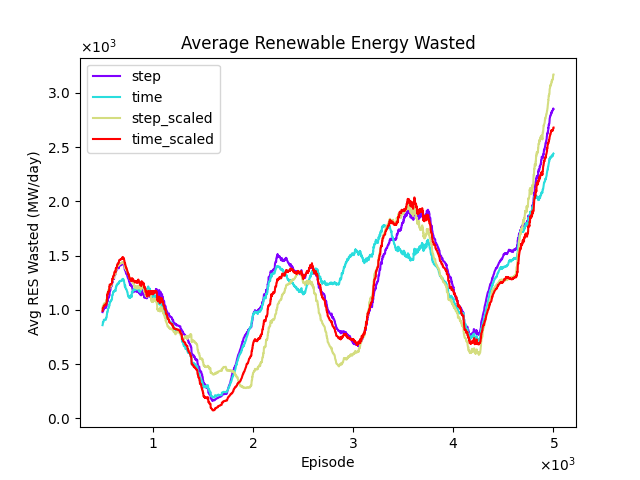
\includegraphics[width=.45\textwidth]{graphs/obs/res_wasted.png}} 
	\caption{Training Results of the Experiments concerning Observation Space.}
	\label{fig:exp-train-obs}
\end{figure}

\begin{table}[ht]
	\centering
	\begin{tabularx}{\textwidth}{|l|X|X|X|X|X|}
		\hline
		\textbf{Model} & \textbf{Avg. Accumulative Reward}& \textbf{Avg. Length (Steps)} & \textbf{Avg Daily Operating Cost (€)} & \textbf{Avg. Renewables Wasted (MW/day)} & \textbf{Total Time (Seconds)}\\
		\hline
		no\_curtail & 133.564 & 515.807  & 531470.223 & 0.0 & 692.832\\
		no\_limit & 128.173 & 403.515 & 585853.240 & 6564.428 & 569.376 \\
		limit\_curtail & 127.951 &  492.732 & 572004.947 & 8877.733 & 678.717 \\
		\hline
	\end{tabularx}
	\caption{Validation Results of the Experiments concerning Limit Infeasible Curtail Actions.}
	\label{fig:exp-val-obs}
\end{table}

\subsection{Curtailment Lower Limit} \label{sec:curtailment-lower-limit}

Beyond the method described in the past subsection, another showed great potential in mitigating the problem related to action space complexity. \par
Remembering the secondary goal of maximising generated renewable energy, the idealisation of a lower bound to restrict the curtailment action space became a possible solution to aid in the model's convergence. In this manner, this condition was included in the implementation in three possible strategies applied solely in the training stage:

\begin{itemize}
	\item No lower bound
	\item Fixed lower bound
	\item Linear decreasing lower bound
	\item Square Root decreasing lower bound
\end{itemize}


\begin{equation}
	y = 1 - \frac{(1 - \underline{P^\text{RES}}) E_\text{train}}{E_\text{decay\_end}}
\end{equation}

\begin{equation}
	y = (1 - \underline{P^\text{RES}}) \sqrt[\alpha]{\frac{E_\text{decay\_end} - E_\text{train}}{E_\text{train}}}
\end{equation}


\begin{comment}
\end{comment}

Results showed in graph GRAPH proved that the introduced curtailment lower bounds considerably increased the model's training performance and convergence, with the square root decay method achieving the overall highest average accumulated reward during validation. Introducing a decay in the lower bound limit implies an enhanced overall performance and survivability of the algorithm.

\section{Rewards Tests} \label{sec:rewards}

Several implementations posed as relevant formulas to describe the reward function of the environment, namely three: Economic Reward, \acp{RES} Penalty Factor Reward and \acp{RES} Bonus Reward. The first considered only the saved cost in non-renewable generators operation, while the second and third accounted for \ac{RES} maximization in a penalty and bonus factor, respectively.
\par

Considering the new parameter introduced by both the Penalty and Bonus Factor rewards, $\beta$, the experiments took into account three distinct values: $\{0.2, 0.4, 0.6\}$.


\par
\begin{comment}
	Graph:
	- Economic Reward
	- Penalty Reward
	- Bonus Reward
	
	Graph:
	- 0.2 pen
	- 0.4 pen
	- 0.6 pen
	- 0.2 bonus
	- 0.4 bonus
	- 0.6 bonus
	
	Do result discussion:
	- Penalty with 0.4 factor was the best
\end{comment}

It's critical to take into account that when evaluating and comparing Reward Functions, the average accumulative reward values have different meanings. Furthermore, other crucial metrics such as the survival rate and the average daily operating cost are favoured.
\par
Results revealed that the proposed implementations were superior to the already defined Economic Reward both in survivability and overall performance of the models. The with the best results were observed in the Penalty Factor Reward with $\beta = 0.2$.

\section{\acp{GNN} Hyperparameter Tuning} \label{sec:gnn-hypertune}

As a key area of this research work, the \ac{GNN} component of the proposed algorithm was given a particular focus in what accounts for hyperparameter tuning. Concrete experiments were devised to assess the performance of different parameter combinations, mainly using the GCN-SAC algorithm. \par

The \ac{GNN} aggregation function plays a fundamental role in the architecture of the solution so the tuning process first focused on this parameter. There are five available types of aggregation schemes:
\begin{itemize}
\item \textbf{Sum} - 
\item \textbf{Max} -
\item \textbf{Min} - 
\item \textbf{Mean} - 
\item \textbf{Mul} - 
\end{itemize}

\begin{comment}
	Validation episodes 295
	119 -> 83
\end{comment}
In a first experiment, five models each with the different types of aggregation functions were trained for 5000 episodes. The main parameters and results can be observed in appendix \ref{appendix}, section \ref{appendix:aggr}. The function that obtained the best average accumulative reward during validation was \texttt{max}, achieving around $4\%$ more than the second placed \texttt{sum} function. Furthermore, this model managed to do better than average in most metrics while simultaneously being outperformed in all of them, which shows the balance between the importance of cost saving while considering the maximization of renewable energy. \par

Regarding the number of \ac{GNN} layers, section \ref{appendix:layers} of appendix \ref{appendix} represents the results from the conducted experiment with this scope. This test considered the \texttt{max} aggregation function and a number of \ac{GCN} layers between $[1,6]$. In contrast with the last experiment, the best model which used a 6-layer \ac{GNN} outperformed the second place with a significant difference of $22.4\%$. This results led to the use of these two parameters in the \ac{GCN} model.




\section{GNN Implementation Comparison} \label{sec:gnn-comparison}

\section{Scalability Tests} \label{sec:scalability-tests}

